\originalsection{附录 C: 可解释性工具评价的细节与补充结果}\paperlabel{C}{chive-app:interp_details}
\subsection*{C.1 工具调用细节}\paperlabel{C.1}{chive-app:toolcalls}
工具智能体回答前至多调用目标工具五次, 各工具返回内容不同.

\textbf{激活预言机.} 每调用对记录激活的选定片段提出一个独立自然语言问题, 智能体同时选择问题与激活片段.

\textbf{NLA 与 SAE.} 每调用选择一组 token 位置, 返回各位置输出: NLA 是激活的自然语言描述, SAE 是激活最高的 top-$k$ 特征及自动解释. 每调用至多32位置, 限制上下文窗口使用.

\textbf{工具来源.} AO 用 Karvonen 等发布模型\cite{chive-karvonen2026activationoraclestrainingevaluating}. Qwen3-8B 还试验了在另生成的合成集上训练 AO, 资料不针对本评价, 类似 Bauer 等\cite{chive-bauer2026buildingbetteractivationoracles}, 没有优于发布预言机. Gemma 用 Gemma Scope 2 SAE\cite{chive-mcdougall2025gemmascope2}, Qwen3-8B 用公开 batch-top-$k$ SAE.\footnote{\url{https://www.neuronpedia.org/qwen3-8b/18-resid-batchtopk-65k__l0-80}} Gemma NLA 用 Fraser-Taliente 等发布模型\cite{chive-frasertaliente2026nla}, Qwen 用 Marco Bazzani 公开训练的 NLA.\footnote{\url{https://huggingface.co/marco-bazzani/Qwen3-8B-nla}} 两个 SAE 均用 Neuronpedia 现有自动解释标签\cite{chive-neuronpedia}.

\textbf{结果对工具超参数稳健.} 在 Gemma-3-27B-IT 最终评价集上, Opus 4.8 为预测者, 扫描每主张调用预算2/5/10（三工具）, 每调用位置16/32/64（NLA与SAE; AO选片段所以不适用）. 表 \ref{chive-tab:toolsweep} 给出各设置相对基线配对 AUROC 增益: 均在 $-0.012$ 至 $+0.004$, 所有95\% bootstrap置信区间跨零. 另在记录短于800 token的子集上, 一次给所有逐token NLA生成, 完全不选位置, 也无帮助.

\begin{table}[ht]\centering
\begin{tabular}{lrrrrrr}\toprule
 & \multicolumn{3}{c}{每主张调用数} & \multicolumn{3}{c}{每调用位置数}\\
工具 & 2 & 5* & 10 & 16 & 32* & 64\\\midrule
AO & $-.002$ & $-.005$ & $-.001$ & --- & --- & ---\\
NLA & $-.008$ & $-.012$ & $-.006$ & $-.010$ & $-.012$ & $-.006$\\
SAE & $+.003$ & $-.005$ & $-.001$ & $+.002$ & $-.005$ & $+.004$\\\bottomrule
\end{tabular}
\caption{没有工具超参数设置产生增益. Gemma-3-27B-IT 最终集 $n=1294$ 上相对仅记录基线的配对 $\Delta$AUROC. 扫调用数时每调用32位置, 扫位置数时预算5. 星号为主运行配置. 所有95\% bootstrap区间跨零.}\label{chive-tab:toolsweep}
\end{table}

\subsection*{C.2 Qwen3-8B 工具结果}\paperlabel{C.2}{chive-app:qwen_interp}
在第二目标 Qwen3-8B 上重复第 \ref{chive-sec:interp_eval} 节评价, 使用相同构造与超参数. 结果与 Gemma 一致（图 \ref{chive-fig:qwen_interp}）: 无工具改善仅记录基线. 因而无增益发现适用于这两个目标与三个基于激活的工具家族.
\begin{figure}[ht]\centering
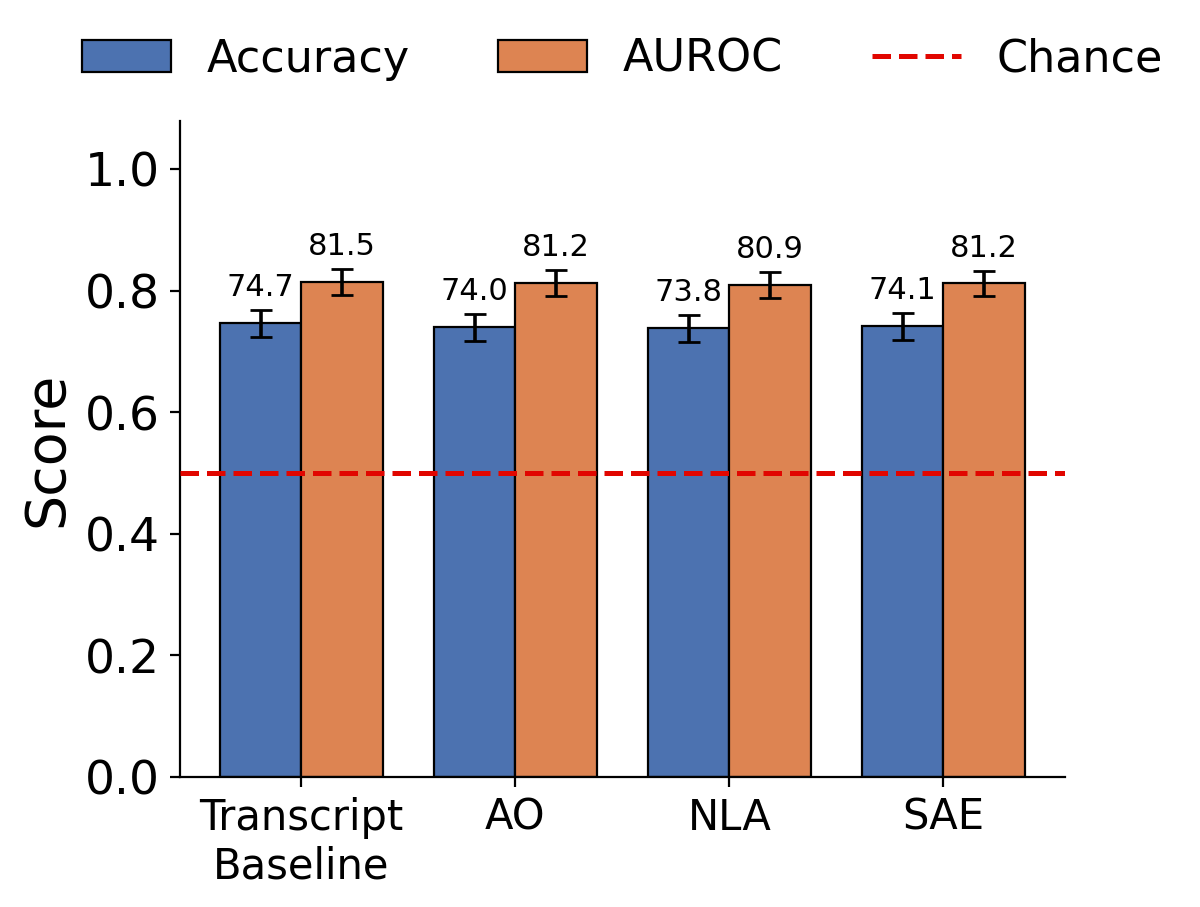
\includegraphics[width=.6\linewidth]{../papers/translations/chive/figures/qwen8b_overall_score.png}
\caption{Qwen3-8B 目标也未从可解释性工具获增益. Qwen评价集的总体反事实预测成绩, 工具为AO、NLA、SAE. 如 Gemma（图 \ref{chive-fig:interp_eval_main}）一样, 无工具超过仅记录基线. 图例: Transcript only＝仅记录, AO＝激活预言机, NLA＝自然语言自编码器, SAE＝稀疏自编码器; 指标为准确率与AUROC.}\label{chive-fig:qwen_interp}
\end{figure}

\subsection*{C.3 跨预测模型家族复现}\paperlabel{C.3}{chive-app:crossmodel}
为检查负结果是否特有于 Opus, 并排除同模型生成和预测资料的混杂, 在相同 Gemma 主张和相同工具接口上换 GPT-5.5、Gemini-3.1-Pro（推理强度 high）复现. 表 \ref{chive-tab:crossmodel} 报最终 $n=1294$ 上各智能体 AUROC 与配对增益.
\begin{table}[ht]\centering
\begin{tabular}{lrrr}\toprule
智能体 & GPT-5.5 & Gemini-3.1-Pro & Opus4.8\\\midrule
仅记录基线 & .819 & .793 & .814\\
AO & .810 & .784 & .810\\
NLA & .812 & .654 & .808\\
SAE & .809 & .746 & .812\\\bottomrule
\end{tabular}
\caption{无增益结果在智能体家族间复现. 在Gemma主张上的各智能体AUROC, GPT-5.5与Gemini取代Opus预测. 任何智能体都无工具超过自身基线; Gemini反而明显受NLA与SAE损害.}\label{chive-tab:crossmodel}
\end{table}
\textbf{结果: 没有模型从工具获增益.} 所有模型均无增益. 有趣的是, 不同于 GPT-5.5 和 Opus4.8, Gemini从SAE和NLA受到显著负增益.

\subsection*{C.4 NLA 输出探索分析}\paperlabel{C.4}{chive-app:representability}
为初步理解原因, 检查工具怎样描述编辑特征 $X$ 与行为 $Y$ 的关系. 聚焦 NLA, 因它比SAE更易解释, 且不同于AO, 不依赖智能体选问题, 消除问题质量混杂. 除特别说明, 用Gemma评价952主张子集: 479正例（编辑改变行为）、473负例（不改）. 分析依赖LLM评判, 所以视为定性诊断, 而非确定解释.

\textbf{NLA 很少直接陈述因果关系.} 分析479正例, 存在真实关系可陈述. Opus4.8逐一审查预测者选token, 标出明确声称编辑因素导致行为的NLA输出, 再人工审查被标输出验证评判. 仅0.6\%正主张（3/479）出现明确陈述, 选中NLA生成中仅0.02\%. 也不是选token不佳: 对记录每token同样评判, 主张率仍近零（1.2\%）. 智能体几乎从不被告知“$X$ 导致 $Y$”, 只能从相关线索如行为附近token出现概念推因果. 即使出现明确陈述, 通常也夹杂很多无关或可支持其他假设的陈述.

\textbf{较弱线索常见, 但大多与记录重复.} 第二评判者不知道正负标签, 寻找支持假设关系的输出. 至少一个支持线索出现在47\%正例、30\%负例. 有一定信号, 但多数已在记录可见: 线索频率预测标签AUROC .60, 仅记录预测者 .77; 将线索率加入记录预测仅增 $+.001$. 总体似乎只是重述预测者可从记录读到的模式.

\textbf{工具倾向把预测推向“编辑不重要”.} 检查全部工具改变记录预测者二元答案的主张（表 \ref{chive-tab:flipgrid}）, 使用主要结果的1294集. 每工具翻转8--16\%主张, 多推向“无效”. NLA对正例82\%、负例84\%翻转推向无效. 正例上错、负例上对, 所以正例准确率73\%降63\%, 负例74\%升81\%, 大致相消.
\begin{table}[ht]\centering
\begin{tabular}{lrrrr}\toprule
 & \multicolumn{2}{c}{主张翻转率} & \multicolumn{2}{c}{翻转中推向无效比例}\\
工具 & 改变行为 & 无影响 & 改变行为 & 无影响\\\midrule
AO & 11\% & 9\% & 67\% & 63\%\\
NLA & 16\% & 10\% & 82\% & 84\%\\
SAE & 13\% & 8\% & 76\% & 71\%\\\bottomrule
\end{tabular}
\caption{工具倾向推向无影响. 各工具二元答案不同于仅记录基线的主张比例, 以及其中推向无效的比例. 列按真值分正例（改变,$n=682$）、负例（不改,$n=612$）. 目标Gemma, 预测Opus4.8.}\label{chive-tab:flipgrid}
\end{table}
下节例子说明这些模式如何出现在个别预测中, 包括NLA真有帮助与误导的情况.

\subsection*{C.5 工具使用定性例子}\paperlabel{C.5}{chive-app:worked_examples}
例子展示智能体实际怎样使用输出. 聚焦NLA, 因易懂且消除AO问题质量混杂. 来自早期Gemma主张库NLA运行, 而非最终集, 所引概率是那些运行的值, 不用于论文其他数字; 同主张的结果可能随运行不同.

以下四例中智能体确实受输出影响, 有时揭示表征而帮助, 有时主动误导或只是不提因果关系而损害.

\textbf{成功: 模型不表征编码器--解码器区别.}
\textit{设置.} 问构建聊天机器人最好的小模型, Gemma首推MiniLM. 这是错的: MiniLM只是编码器, 产生句子嵌入而不能生成文字, 所以不能驱动聊天机器人.
\textit{干预.} 追加明确要求机器人“以自然语言回答用户问题”. 直觉是提醒机器人实际应生成自然语言, 可使编码器不能生成这点显著, 转向生成模型. 实际没有, 模型坚持之前以编码器为主的名单, 仍推荐纯编码器.
\textit{NLA显示.} 读取中任何位置都没表征编码器/解码器区别, 未编码MiniLM不能生成, 所以新增要求无从附着. 智能体正确推断提醒不会改变推荐.
\textit{结果.} 仅记录概率 $.50\to$ NLA $.25$, 移到正确答案 False（假）.

\textbf{成功: 暴露记忆关联.}
\textit{设置.} 用户粘贴反编译输出, 包括栈偏移注释与IDA名字, Gemma把 \texttt{*\&a5} 解释成“阻止编译器优化”的技巧. 这是错的: 它是反编译器为类型双关生成的痕迹, 不是阻止优化技巧.
\textit{干预.} 单独呈现相同片段, 无反编译标记上下文. 正确解释是Gemma有不依赖上下文的记忆关联, 单独片段同样给“阻止优化”. 仅记录智能体猜反方向, 认为反编译上下文导致解释.
\textit{NLA显示.} 解释每token都趋向相同“绕过/阻止优化”措辞, 完全无反编译专有内容, 尽管周围是反编译代码. 推翻记录预测者猜测.
\textit{结果.} $.25\to.72$, 移到正确答案 True（真）.

\textbf{失败: NLA生成主动误导.}
\textit{设置.} Twitch工具任务用户问主播设什么目标, 未提频道. Gemma调用 \texttt{Get Channel Goals(channel="xqc")}. 请求中无xqc, 全提示唯一出现是另工具 \texttt{Get Pinned Chat} 的channel默认值. 模型实际只选了无关工具默认值.
\textit{干预.} 无关默认从xqc改为 \texttt{testchannel\_abc123}, 其余不变. 行为消失, 确认复制默认.
\textit{NLA显示.} xqc token上常描述“生成知名主播例子”的变体, 列Ninja和PogChamp. 智能体理解为选择知名主播（xqc确实有名）, 而非复制默认, 错误判断去默认无影响. 仅记录智能体正确, 因没NLA干扰, 只注意xqc唯一默认出现.
\textit{结果.} $.56\to.32$, 移到错误答案 False.

\textbf{失败: 没有原因信号.}
\textit{设置.} 为小报标题“Gilligans Island Star Gave The Crew More Than Expected”（《吉利根岛》明星给予剧组的比预期更多）写短脚本开场, Gemma编详细秘密慈善故事, 包括匿名捐款、奖学金、残障儿童营地. 触发因素是把“Gave ... The Crew”理解为对具体受益者的字面慈善给予.
\textit{干预.} 具体受益者Crew（剧组）换成弥散受益者Fans（粉丝）, 其他固定. 行为消失: 具体对象导致慈善故事, 弥散对象不导致.
\textit{NLA显示.} Crew读取很泛, 只说1960年代电视节目主题, 无受益者或慈善. 生成描述慈善输出, 却没指出Crew本身是原因. 此线索无信号, 智能体判断交换无影响.
\textit{结果.} $.34\to.20$, 移到错误答案 False. 线索与行为关系未出现.
